\documentclass[11pt,a4paper]{article}

\usepackage{amsmath,amssymb,amsbsy}
\usepackage{bm}
\usepackage[margin=1in]{geometry}
\usepackage[numbers,sort&compress]{natbib}
\usepackage{tikz}
\usetikzlibrary{arrows.meta}
\usepackage[colorlinks=true,linkcolor=blue,citecolor=blue,urlcolor=blue]{hyperref}

\newcommand{\grad}{\bm{\nabla}}
\newcommand{\rr}{\mathbf{r}}
\newcommand{\svec}{\mathbf{s}}
\newcommand{\RR}{\mathbf{R}}
\newcommand{\nn}{\mathbf{n}}
\newcommand{\Bg}{\mathbf{B}_{\mathrm{g}}}
\newcommand{\Eg}{\mathbf{E}_{\mathrm{g}}}
\newcommand{\half}{\tfrac{1}{2}}

\title{Internal degrees of freedom in wave-mechanical structure formation:\\
vorticity, spin, and a rotor extension of the Schr\"odinger--Poisson system}
\author{Edward A. Thomson}
\date{Working paper, 2026}

\begin{document}
\maketitle

\begin{abstract}
\noindent
Wave-mechanical methods describe cold and ultralight dark matter as a complex scalar
field evolving under the Schr\"odinger--Poisson equations, with $|\psi|^2$ the mass
density and the phase gradient the velocity. This description is intrinsically
irrotational and structureless: it admits neither vorticity in the bulk flow nor
internal angular momentum for extended objects. This paper sets out a programme to
endow wave-mechanical structure formation with internal degrees of freedom. For
vorticity we adopt a gravitational vector potential from the weak-field
(gravitoelectromagnetic) limit of general relativity, coupled to the wavefunction by
minimal coupling. For spin we show that the leading coupling of an extended body to an
external gravitational field is through its quadrupole moment and the tidal tensor,
yielding a torque that spins up non-spherical objects under purely Newtonian gravity.
We argue that the natural internal variable is a rotor (a unit quaternion), of which
the two-component Pauli spinor is the axisymmetric special case, and we propose a
multicomponent Schr\"odinger--Poisson system that carries this internal state and
reduces to the scalar theory when it is switched off. We give an implementation roadmap
and identify the open theoretical problems. The formulation is presented as a direction
of travel: the geometric and multipole content is established, while the
self-consistent field equations and their coupling constants remain to be derived and
tested.
\end{abstract}

\section{Introduction}
\label{sec:intro}

The wave-mechanical approach to cosmological structure formation replaces the discrete
particles of an $N$-body simulation with a single complex scalar field $\psi$. Through
the Madelung transform \citep{madelung1927} the Schr\"odinger equation is equivalent to
a set of fluid equations, so that $|\psi|^2$ plays the role of a mass density and the
gradient of the phase plays the role of a velocity field. Widrow and Kaiser
\citep{widrow_kaiser1993} proposed using this equivalence as a numerical method for
collisionless matter, and the idea has since become central to the study of ultralight
or ``fuzzy'' dark matter, in which the field is physical rather than a numerical device
\citep{hu2000,schive2014,mocz2017}. The same formalism underlies the wave-mechanical
perspective on large-scale structure developed by Short \citep{short2007}, Johnston,
Lasenby and Hobson \citep{johnston2010}, and in the present author's thesis, whose
solver and results this paper builds upon.

The strength of the wave-mechanical description is also the origin of the limitation we
address here. Because the velocity is the gradient of a scalar phase,
$\mathbf{v} = \nu\,\grad\arg\psi$, the flow it represents is potential flow: it is
irrotational wherever the wavefunction is smooth and non-zero. Vorticity can appear
only at the nodes of $\psi$, where the phase is undefined and the density vanishes.
Equally, a single scalar field has no internal orientation: it cannot represent an
extended object that carries intrinsic angular momentum, nor the torque that a tidal
field exerts on such an object. Yet real structures rotate, haloes acquire angular
momentum through tidal torquing, and galaxies within clusters show alignment effects.
If wave mechanics is to be a complete language for structure formation, and not only
for the smooth potential-flow regime, it needs a controlled way to carry these internal
degrees of freedom.

This paper describes a programme to provide them. It has two strands, corresponding to
the two physically distinct notions that a scalar field omits.

\begin{itemize}
  \item \emph{Vorticity}, meaning circulation in the bulk velocity field. We generate
  it by enlarging the force law with a gravitational vector potential, taken from the
  gravitoelectromagnetic (GEM) weak-field limit of general relativity
  \citep{mashhoon2003}, and coupled to the wavefunction by the same minimal coupling
  used for a charged particle in a magnetic field \citep{watanabe2000}.
  \item \emph{Spin}, meaning internal angular momentum of an extended object. We show
  that this arises already under Newtonian gravity, through the coupling of the object's
  quadrupole moment to the external tidal tensor, and we carry it in wave mechanics by
  promoting the wavefunction to a field that also depends on an internal orientation
  variable.
\end{itemize}

The central claim on the spin side is geometric. The coupling of an extended body to
gravity is to the rank-two tidal tensor, not to a rank-one field, so the natural
internal variable is not a two-component spinor but a \emph{rotor}: a unit element of
the even Clifford algebra $\mathrm{Cl}_3^{+}$, isomorphic to the unit quaternions,
which represents a full three-dimensional orientation. The Pauli-like equation that one
might write by analogy with quantum spin then reappears as the special case of an
axisymmetric body, not as the fundamental description. Recognising this fixes both the
degree-of-freedom counting and the choice of coupling.

We are explicit about status. The multipole and tidal-torque content of
Sections~\ref{sec:spin} and \ref{sec:rotor} is standard and reliable. The
gravitoelectromagnetic route of Section~\ref{sec:vorticity} rests on an established
weak-field theory. The self-consistent multicomponent Schr\"odinger--Poisson system of
Section~\ref{sec:multicomponent} is a target rather than a result: its internal
Hamiltonian, the measure on the orientation space, and the coupling constants remain to
be derived, and the reductions to the scalar theory need to be checked against the
comoving formulation of the thesis before any implementation. Section~\ref{sec:roadmap}
sets out how that programme could be carried through.

\section{Wave-mechanical structure formation}
\label{sec:background}

We recall the scalar system that the extensions of this paper build on. In physical
variables a single wavefunction $\psi(\mathbf{x},t)$ evolves under the
Schr\"odinger--Poisson equations,
%
\begin{equation}
  i\hbar\,\frac{\partial \psi}{\partial t}
  = \left[ -\frac{\hbar^2}{2m}\nabla^2 + m\,\Phi \right]\psi,
  \qquad
  \nabla^2 \Phi = 4\pi G\,\rho, \qquad \rho = m\,|\psi|^2 .
  \label{eq:sp-physical}
\end{equation}
%
Writing $\psi = \sqrt{\rho/m}\,\exp(i\theta)$ and separating real and imaginary parts
returns the continuity and Euler equations of a fluid with velocity
$\mathbf{v} = (\hbar/m)\grad\theta$ and an additional ``quantum pressure'' term
\citep{madelung1927}. The parameter that controls the correspondence is
$\nu = \hbar/m$, which sets both the de~Broglie scale and, on a grid of $N$ points, the
largest velocity the phase can represent before it aliases,
$v_{\max} = \nu\,\pi\,N$. Resolving the velocity field therefore requires $\nu N$ to be
large enough; this is the origin of the resolution constraint identified in the
accompanying code and thesis, and it is the reason the method is exact for smooth
potential flow but says nothing, by itself, about rotational or internal motion.

In the rescaled comoving variables used for the cosmological runs (comoving coordinate
$\mathbf{y}$, comoving wavefunction $\chi$, comoving potential $U$, and a dimensionless
parameter $\mathcal{L}$), the same system reads, schematically,
%
\begin{equation}
  2 i \mathcal{L}\left[\Omega_{m0} + (1-\Omega_{m0})a^3\right]^{1/2}
  \frac{\partial \chi}{\partial \ln a}
  = \left[ -\nabla_{\mathbf{y}}^2 + 3\,\Omega_{m0}\,\mathcal{L}^2\,U \right]\chi,
  \qquad
  \nabla_{\mathbf{y}}^2 U = \chi\chi^{\ast} - 1 ,
  \label{eq:sp-comoving}
\end{equation}
%
with the Einstein--de~Sitter case recovered by $\Omega_{m0}=1$. Both
\eqref{eq:sp-physical} and \eqref{eq:sp-comoving} are scalar: $\psi$ and $\chi$ carry a
density and a phase and nothing else. The remainder of this paper asks what minimal
additional structure is needed to represent vorticity and spin, and how to add it
without disturbing the parts of the theory that already work.

\section{Vorticity via gravitoelectromagnetism}
\label{sec:vorticity}

Throughout the standard setting the peculiar velocity is generated from a scalar
potential and is therefore initially irrotational,
$\grad\times\mathbf{F}_{\mathrm{g}} = \grad\times\grad\phi_{\mathrm{g}} \equiv 0$, so
Kelvin's circulation theorem forbids the growth of vorticity in the smooth
pre-shell-crossing regime. Within wave mechanics the only candidate sites for
circulation are the nodes of $\psi$, where the density vanishes and the phase is
singular. To generate vorticity dynamically, rather than merely to diagnose singular
behaviour, the force law itself must be enlarged so that its curl need not vanish.

A phenomenological vector potential would do this but would be arbitrary. A physically
motivated route is gravitoelectromagnetism, the weak-field, slow-motion limit of
general relativity in which the field equations take a form analogous to Maxwell's
\citep{mashhoon2003}. One introduces a gravitoelectric field $\Eg$, reducing to the
Newtonian field in the static limit, and a gravitomagnetic field $\Bg$ sourced by mass
currents,
%
\begin{equation}
  \grad\cdot\Eg = -4\pi G \rho_{\mathrm{g}}, \qquad
  \grad\cdot\Bg = 0, \qquad
  \grad\times\Eg = -\frac{\partial \Bg}{\partial t}, \qquad
  \grad\times\Bg = -\frac{4\pi G}{c^2}\mathbf{J}_{\mathrm{g}}
  + \frac{1}{c^2}\frac{\partial \Eg}{\partial t},
\end{equation}
%
with $\rho_{\mathrm{g}}$ the mass density (identified with $m|\psi|^2$) and
$\mathbf{J}_{\mathrm{g}}$ the mass-current density (related to the probability current
that already defines the velocity). The associated Lorentz-like force is
%
\begin{equation}
  \mathbf{F}_{\mathrm{g}} = m\left( \Eg + 2\,\mathbf{v}\times\Bg \right),
  \label{eq:gem-lorentz}
\end{equation}
%
where the factor of two on the gravitomagnetic term reflects the spin-two character of
the gravitational field. The gravitomagnetic force acts perpendicular to the velocity;
it is not curl-free, so vorticity generation is no longer forbidden.

This field enters a Schr\"odinger-like evolution by minimal coupling, exactly as for a
charged particle in a magnetic field. Watanabe and Tsukada \citep{watanabe2000} write
%
\begin{equation}
  i\hbar\frac{\partial}{\partial t}\psi
  = -\frac{\hbar^2}{2m}\left(\grad - \frac{ie}{\hbar}\mathbf{A}\right)^2\psi,
\end{equation}
%
and show that the evolution can be handled efficiently with splitting operators; a
spatially uniform vector potential changes only the phase, while a spatially varying
$\mathbf{A}(\mathbf{x})$ also modifies the kinetic operator. In the gravitational case
the charge $e$ is replaced by the mass $m$ and $\mathbf{A}$ by the gravitomagnetic
potential $\mathbf{A}_{\mathrm{g}}$, with $\Bg = \grad\times\mathbf{A}_{\mathrm{g}}$.

That the ingredients are already present can be checked without modifying the dynamics.
The gravitomagnetic field of a rotating mass distribution is a dipole,
%
\begin{equation}
  \Bg = \frac{G}{2c^2 r^3}\left[ \mathbf{L} - 3(\mathbf{L}\cdot\hat{\mathbf{r}})
  \hat{\mathbf{r}} \right],
  \qquad
  \mathbf{L} = \sum_j m_j\,(\rr_j\times\mathbf{v}_j),
\end{equation}
%
and evaluating $\mathbf{L}$ and $\Bg$ on the $N$-body outputs used elsewhere in the
thesis gives a non-zero field whose ratio to the Newtonian force falls with time and is
suppressed by $v^2/c^2$. The conclusion is not that the effect is dynamically large in a
cosmological setting, but that the field is not identically zero in principle, so that a
self-consistent GEM extension is well posed. Including it in the equations of motion,
whether in an $N$-body or a wave-mechanical code, is the natural next step for the
vorticity strand.

\section{Spin of structured objects}
\label{sec:spin}

The second strand concerns internal angular momentum rather than bulk circulation. A
purely scalar Newtonian potential cannot produce a gravitomagnetic force, but it can
exert a torque on a body of finite extent when the field varies across it. Spin can
therefore arise in a model that remains irrotational at the level of the centre-of-mass
flow, which is why it must be treated separately from vorticity.

Consider a super-particle: an unresolved extended object with internal mass
distribution $\rho(\svec)$, where $\svec$ is the displacement from the centre of mass
$\RR$. Following the multipole treatment of an extended body in an external field
\citep{jackson1998}, the interaction energy with an external potential
$\phi_{\mathrm{ext}}$ is
%
\begin{equation}
  U(\RR) = \int \rho(\svec)\,\phi_{\mathrm{ext}}(\RR+\svec)\,d^3 s
  = M\,\phi_{\mathrm{ext}}
  + d_i\,\partial_i \phi_{\mathrm{ext}}
  + \half\,Q_{ij}\,\partial_i\partial_j \phi_{\mathrm{ext}}
  + \cdots,
  \label{eq:multipole}
\end{equation}
%
with
%
\begin{equation}
  M = \int \rho\,d^3 s, \qquad
  d_i = \int \rho\,s_i\,d^3 s, \qquad
  Q_{ij} = \int \rho\,s_i s_j\,d^3 s .
\end{equation}
%
For a gravitational mass distribution in its own centre-of-mass frame the dipole moment
vanishes, $d_i = 0$, because all mass ``charges'' have the same sign; there is no
gravitational analogue of the electric dipole. The first non-trivial coupling of the
internal structure to the external field is therefore at quadrupole order, through the
tidal tensor $T_{ij} = \partial_i\partial_j\phi_{\mathrm{ext}}$. This is the key
physical point: a meaningful spin coupling must be built from the tidal tensor and the
quadrupole moment, not from a gravitational dipole that is identically zero.

Writing the local force density as $-\rho(\svec)\,\grad\phi_{\mathrm{ext}}(\RR+\svec)$ and
expanding the gradient to first order in $\svec$,
%
\begin{equation}
  \grad\phi_{\mathrm{ext}}(\RR+\svec) \approx
  \grad\phi_{\mathrm{ext}}(\RR) + T\cdot\svec ,
\end{equation}
%
the zeroth-order term produces no torque because the dipole vanishes, and the leading
torque about the centre of mass is
%
\begin{equation}
  \tau_i = -\,\epsilon_{ijk}\,T_{k\ell}\,Q_{j\ell}.
  \label{eq:torque}
\end{equation}
%
Equation~\eqref{eq:torque} is the clean Newtonian statement of the mechanism: a
non-spherical body spins up because its quadrupole tensor is not aligned with the tidal
tensor. It carries no spurious numerical factors; the corresponding dumbbell equation
of motion in the thesis chapter has been corrected accordingly.

\begin{figure}[t]
\centering
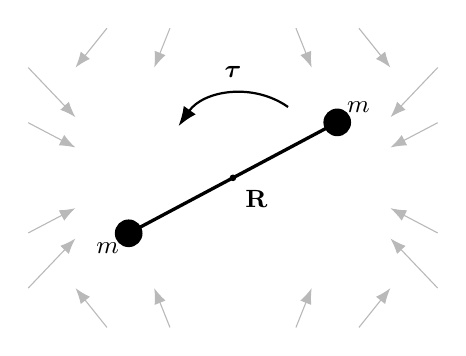
\begin{tikzpicture}[scale=1.0]
  % tidal field arrows (converging vertically, diverging horizontally)
  \foreach \y in {-1.4,-0.7,0.7,1.4}{
    \draw[gray!55,-{Latex[length=2mm]}] (-2.6,\y) -- (-2.0,{0.55*\y});
    \draw[gray!55,-{Latex[length=2mm]}] ( 2.6,\y) -- ( 2.0,{0.55*\y});
  }
  \foreach \x in {-1.6,-0.8,0.8,1.6}{
    \draw[gray!55,-{Latex[length=2mm]}] (\x, 1.9) -- ({1.25*\x}, 1.4);
    \draw[gray!55,-{Latex[length=2mm]}] (\x,-1.9) -- ({1.25*\x},-1.4);
  }
  % dumbbell, tilted
  \def\ang{28}
  \coordinate (c) at (0,0);
  \coordinate (m1) at ({1.5*cos(\ang)},{1.5*sin(\ang)});
  \coordinate (m2) at ({-1.5*cos(\ang)},{-1.5*sin(\ang)});
  \draw[very thick] (m2) -- (m1);
  \fill (m1) circle (5pt); \fill (m2) circle (5pt);
  \node at (0,0) [below right=1pt] {\small $\RR$};
  \fill (c) circle (1.2pt);
  \node at (m1) [above right] {\small $m$};
  \node at (m2) [below left] {\small $m$};
  % torque arrow
  \draw[thick,-{Latex[length=2.5mm]}] (0.7,0.9) arc (55:145:1.0);
  \node at (0,1.35) {\small $\boldsymbol{\tau}$};
\end{tikzpicture}
\caption{A quadrupolar (dumbbell) super-particle in an external tidal field $T_{ij}$
(grey arrows). The gravitational dipole vanishes, so there is no net dipole force, but
the misalignment between the object's quadrupole tensor and the tidal tensor produces a
torque $\boldsymbol{\tau}$ about the centre of mass $\RR$, spinning the object up under
purely Newtonian gravity.}
\label{fig:dumbbell}
\end{figure}

For the simplest illustration, two equal masses at $\svec^{(1)}=(+x,0,0)$ and
$\svec^{(2)}=(-x,0,0)$ (Figure~\ref{fig:dumbbell}) have zero dipole moment but a non-zero
quadrupole $Q_{ij} = 2mx^2\,\mathrm{diag}(1,0,0)$, and as the pair rotates the
quadrupole stays non-zero. It is the minimal system with non-trivial tidal coupling.
For an axisymmetric body with symmetry axis $\nn$ one may write
%
\begin{equation}
  Q_{ij} = q\,n_i n_j, \qquad
  U_{\mathrm{spin}} = \half\,q\,n_i T_{ij} n_j, \qquad
  \boldsymbol{\tau} = -\,q\,\nn\times(T\cdot\nn),
  \label{eq:axisym}
\end{equation}
%
which is a single internal degree of freedom, the orientation of $\nn$, that can be
evolved directly.

\section{The Pauli reduction and its limits}
\label{sec:pauli}

Because wave mechanics already accommodates multi-component fields, it is tempting to
carry the internal orientation in a spinor and to couple it in the manner of the Pauli
equation. Using the isomorphism between the Clifford algebra of three-dimensional space
and the complex $2\times2$ matrices, $\mathrm{Cl}_3 \cong \mathrm{Mat}(2,\mathbb{C})$
with $\mathbf{e}_i \leftrightarrow \sigma_i$ \citep{lounesto2001}, a body axis
$\mathbf{d}=d_i\mathbf{e}_i$ maps to the Hermitian matrix $d_i\sigma_i$, and the
dipole-order interaction energy takes the form
%
\begin{equation}
  U = \mathbf{B}\cdot\mathbf{S}
  = \begin{pmatrix} B_z d_z & B_x d_x - i B_y d_y \\
                    B_x d_x + i B_y d_y & -B_z d_z \end{pmatrix},
  \qquad B_i = \partial_i\phi,
\end{equation}
%
which is Hermitian, as required, and yields a Pauli-like equation
%
\begin{equation}
  i\hbar\frac{\partial}{\partial t}\psi_{\pm}
  = \left( -\frac{\hbar^2}{2m}\nabla^2 + mV \right)\mathbf{I}\,\psi_{\pm}
  - \mu\,\mathbf{B}\cdot\mathbf{S}\,\psi_{\pm}
\end{equation}
%
for a two-component wavefunction $\psi_{\pm}$, reducing to two independent
Schr\"odinger equations when the coupling is switched off \citep{johnston2010}. In this
construction the coupling constant is fixed by analogy, $\mu = m$, rather than derived.

There are two reasons not to take this as the fundamental description. First, the
gravitational coupling is to the rank-two tidal tensor $T_{ij}$, not to a rank-one
field, so a linear $\mathbf{B}\cdot\bm{\sigma}$ term is not the natural object; the
quadrupole form \eqref{eq:torque} is. Second, and more concretely, a two-component
spinor does not carry enough information to orient a general body. A complex two-spinor
has four real parameters; removing the overall norm and phase leaves two physical
degrees of freedom, a point on the Bloch sphere, which is a single axis direction
$n_i = \xi^{\dagger}\sigma_i\xi / \xi^{\dagger}\xi$. That is exactly an axisymmetric
body, $Q_{ij}=q\,n_i n_j$, and no more. A general triaxial object needs three
rotational degrees of freedom and, in addition, two trace-free shape parameters to fix
the principal quadrupole values. The two-spinor encodes a preferred axis but not a
complete body frame, and cannot distinguish rotations about that axis. It is a correct
but partial model, adequate for a dumbbell and inadequate for a triaxial halo.

\section{Rotor-valued internal states}
\label{sec:rotor}

The variable that does carry a full orientation is a rotor. In three dimensions the
even subalgebra $\mathrm{Cl}_3^{+}$ is isomorphic to the quaternions $\mathbb{H}$, and
unit rotors double-cover the rotation group $SO(3)$ \citep{lounesto2001,mtw1973}. A
rotor $R$ satisfies $R\tilde{R}=1$, where $\tilde{R}$ is the reversion, and it rotates a
body-fixed orthonormal frame $\{\mathbf{e}_a\}$ into lab-frame axes
%
\begin{equation}
  \mathbf{E}_a = R\,\mathbf{e}_a\,\tilde{R}, \qquad a = 1,2,3 .
\end{equation}
%
A body with principal-frame quadrupole
$Q^{\mathrm{body}} = \mathrm{diag}(q_1,q_2,q_3)$ then has lab-frame quadrupole
%
\begin{equation}
  Q_{ij}(R) = \sum_{a=1}^{3} q_a\,(\mathbf{E}_a)_i (\mathbf{E}_a)_j
  = \bigl(\mathcal{R}(R)\,Q^{\mathrm{body}}\,\mathcal{R}(R)^{\mathsf{T}}\bigr)_{ij},
  \label{eq:Qrotor}
\end{equation}
%
where $\mathcal{R}(R)\in SO(3)$ is the rotation associated with $R$, and the interaction
keeps the quadrupole form
%
\begin{equation}
  U_{\mathrm{int}}[R] = \half\,Q_{ij}(R)\,T_{ij}.
  \label{eq:Uint-rotor}
\end{equation}
%
This is the honest generalisation of the axisymmetric model \eqref{eq:axisym}: the
internal variable is now a full orientation state, and the force and torque continue to
descend from the tidal coupling rather than from a guessed linear term. The Pauli
two-spinor of Section~\ref{sec:pauli} is recovered by restricting $R$ to rotations of a
single axis, that is, by taking $Q^{\mathrm{body}}=\mathrm{diag}(q,0,0)$ and reading off
$\nn$ from the corresponding spinor. The Clifford and Pauli-matrix representations
remain useful as computational tools, but they no longer carry the physics unaided: the
Hamiltonian comes from \eqref{eq:multipole} and \eqref{eq:Uint-rotor}, not from the
representation.

\section{A multicomponent Schr\"odinger--Poisson system}
\label{sec:multicomponent}

We now propose how the internal state enters the wave-mechanical evolution. The proposal
is schematic: the equations below fix the structure that a self-consistent theory should
have, but the internal Hamiltonian, the measure over orientation space, and the coupling
constants remain to be derived, and the reductions should be verified against
\eqref{eq:sp-comoving}.

Promote the scalar field to a field that also depends on an internal orientation
coordinate $R$, and let the density be an integral over that coordinate. In physical
variables,
%
\begin{align}
  i\hbar\,\frac{\partial \Psi}{\partial t}
  &= \left[ -\frac{\hbar^2}{2m}\nabla^2 + m\Phi
  + \hat{H}_{\mathrm{int}}\bigl(T[\Phi],R\bigr) \right]\Psi,
  \label{eq:mc-physical}\\
  \nabla^2\Phi &= 4\pi G\,m \int \Psi^{\dagger}(\mathbf{x},t,R)\,\Psi(\mathbf{x},t,R)\,
  d\mu(R),
\end{align}
%
where the internal Hamiltonian is built from the self-consistent tidal tensor
$T_{ij}[\Phi] = \partial_i\partial_j\Phi$ and encodes the quadrupole coupling
\eqref{eq:Uint-rotor}. The essential property is that when the internal state
factorises, $\Psi(\mathbf{x},t,R) = \psi(\mathbf{x},t)\,\Xi(R,t)$, with unit norm
$\int \Xi^{\dagger}\Xi\,d\mu(R) = 1$, and $\hat{H}_{\mathrm{int}}$ is absent or frozen,
the density reduces to $\rho = m|\psi|^2$ and \eqref{eq:mc-physical} collapses to the
scalar Schr\"odinger--Poisson system \eqref{eq:sp-physical}. The construction is an
extension of the thesis framework, not a replacement for it.

The same structure written in the comoving variables of \eqref{eq:sp-comoving} adds
$\hat{H}_{\mathrm{int}}(\mathcal{T}[U],R)$ inside the bracket, with comoving tidal tensor
$\mathcal{T}_{ij}[U] = \partial_{y_i}\partial_{y_j}U$, and replaces $\chi\chi^{\ast}$ in
the Poisson source by $\int \Psi^{\dagger}\Psi\,d\mu(R)$. The scalar comoving system is
recovered under the same factorisation and unit-norm condition. Fixing the precise form
of $\hat{H}_{\mathrm{int}}$ and $d\mu(R)$, and checking the normalisation against
Chapter~5 of the thesis, are the first theoretical tasks of the programme.

\section{Implementation roadmap}
\label{sec:roadmap}

The formulation is designed to reuse the existing spectral, operator-split solver. The
translational part of \eqref{eq:mc-physical} is unchanged and evolves with the same
split-operator kinetic and potential steps. The internal part is a small additional
factor in the splitting, acting on the orientation state at fixed position. A practical
route is a ladder of increasing self-consistency.

\begin{enumerate}
  \item \emph{Fixed external tide, one body.} Evolve a single rotor (or its
  axisymmetric spinor reduction) in a prescribed tidal tensor and verify the torque law
  \eqref{eq:torque} against the analytic rigid-body solution. This tests the internal
  Hamiltonian in isolation.
  \item \emph{Self-consistent pair.} Couple two super-particles through the Poisson
  solve, so that each provides the tidal field of the other, and check angular-momentum
  bookkeeping and the recovery of the scalar limit when the internal coupling is
  switched off.
  \item \emph{Cosmological field.} Carry the internal state on the full comoving grid,
  using the multicomponent Poisson source, and measure the statistics of induced spin
  against the tidal-torque expectation.
\end{enumerate}

At each stage the diagnostics are the conserved quantities (total mass, total angular
momentum) and the reduction to the scalar solver when $\hat{H}_{\mathrm{int}}\to 0$. The
vorticity strand of Section~\ref{sec:vorticity} can be developed in parallel, since
minimal coupling of the gravitomagnetic potential also fits the splitting scheme
\citep{watanabe2000}; combining the two would allow spin-orbit effects to be studied,
though that is a later goal.

\section{Discussion}
\label{sec:discussion}

The programme is deliberately conservative in its physics and ambitious only in its
scope. Each ingredient is either standard (the multipole expansion and tidal torque,
the weak-field GEM equations) or a faithful reorganisation of the thesis proposal (the
rotor internal state generalising the Pauli spinor). What is new is the claim that these
can be assembled into a single multicomponent Schr\"odinger--Poisson system that carries
internal degrees of freedom and reduces cleanly to the scalar theory.

Whether the effects matter dynamically is an open question, and the honest expectation
is that they are small in the smooth cosmological regime and largest where tides are
strong or objects are compact and rapidly forced. Even where the dynamical effect is
small, the framework has diagnostic value: it gives a principled way to read intrinsic
spin and its alignment out of a wave-mechanical simulation, quantities that a scalar
field cannot represent at all. It also connects the wave-mechanical programme to the
broader effort to understand the relationship between the Schr\"odinger method and its
$N$-body and fluid limits \citep{widrow_kaiser1993,uhlemann2014}, now extended beyond
the point-particle idealisation.

\section{Conclusion}
\label{sec:conclusion}

We have set out a direction for wave-mechanical structure formation: to give it the
internal degrees of freedom that a scalar wavefunction lacks. Vorticity is to be
generated by a gravitational vector potential from the weak-field limit of general
relativity, coupled by minimal coupling. Spin is to be carried by a rotor-valued
internal state, coupled to the tidal tensor through the quadrupole moment, with the
familiar Pauli spinor recovered as the axisymmetric special case. The two strands come
together in a multicomponent Schr\"odinger--Poisson system that reduces to the scalar
theory when the internal state is switched off. The geometric and multipole content of
the proposal is established; the self-consistent field equations, their coupling
constants, and their numerical behaviour remain to be worked out. The roadmap of
Section~\ref{sec:roadmap} is how we intend to do that.

\bibliographystyle{plainnat}
\bibliography{refs}

\end{document}
